\documentclass[../main.tex]{subfiles}

\graphicspath{{pictures/}{../pictures/}}

\chapterimage{chapter_head_8.pdf} % Chapter heading image

\begin{document}
	%----------------------------------------------------------------------------------------
	%	Data Structures
	%----------------------------------------------------------------------------------------
	\chapter{Data Structures}
	As you've seen with C up until this point, you tend to have to build everything yourself.  This is why understanding data structures is an important skill to have.  In the following sections, we'll discuss \textit{linked-lists}, \textit{queues}, \textit{stacks}, \textit{binary search tree}, and \textit{hashtable}.  There are multiple ways that they could be constructed.  The following examples have been made to store data of type \textit{void *} so that they can be used with any data type.  An understanding of pointers and dynamic memory will be essential when building and working with custom data structures.
	
	\section{Linked-List}
	A \textit{linked-list} is a fairly simple data structure where one node points to the next node.  You may see a \textit{singly linked-list}, \textit{doubly linked-list}, and even a \textit{circly linked-list}.  We'll keep it simple with a \textit{singly linked-list}.\\
	
	\lstinputlisting[caption={\lstname}, label={lst:ll_header}]{src/09-ll.h}
	
	In the header file we have two \textit{structs}, \textit{ll\_t} and \textit{node\_t}.  The \textit{ll\_t struct} will contain the first \textit{node\_t} which is called the "head".  The "next" pointer in each \textit{node\_t struct} will point to the next node in the list unless there are no additional nodes.  In that case, the "next" pointer will be \textit{NULL}.  Again, there are a handful of different ways you could construct a linked-list.  However, the basis premise is one node points to the next node.
	
	\begin{figure}[h]
		\centering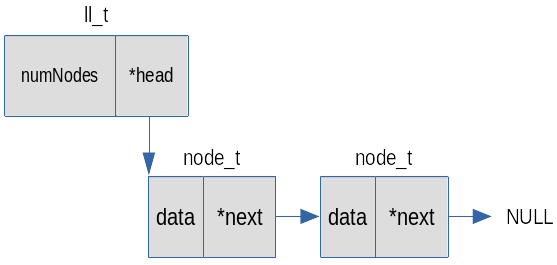
\includegraphics[scale=0.5]{linkedlist.png}
		\caption{Linked-List}
		\label{fig:linked_list}
	\end{figure}

	In this implementation I am even keeping track of the number of nodes by having a \textit{numNodes} entry in the \textit{ll\_t struct}.  This isn't necessary nor is it probably common.  However, you are free to customize your implementation to your application.  Maybe periodically looking up how many nodes are in my list is something my program needs to be aware of.  If this wasn't something I was already keeping track of, I would have to traverse the entire list to count the nodes each time I needed to know.  
	
	We can also see in the header file that I have implemented a number of functions that will serve sat the API to interact with the linked-list.  In this case, we have functions to initially create the list, destroy the list, add a node to the list, remove a node from the list, and even print our list.  Because we are storing the data as \textit{void *}, the implementation requires the passing in of function pointers that know how to handle the particular data type that we've stored.  
	
	Let's look to see how all of this is implemented:\\

	\lstinputlisting[caption={\lstname}, label={lst:ll}]{src/09-ll.c}
	
	\subsection{createList}
	On line 8 of \textit{createList} you can see that I use \textit{calloc} to dynamically allocate space for the \textit{ll\_t struct}.  This means that \textit{numNodes} will be set to zero and \textit{head} will be set to \textit{NULL}.
	
	\subsection{destroyList}
	On line 13 we begin the \textit{destroyList} function.  Here we see the list is passed in as a pointer to a pointer.  This is so that we can \textit{NULL} out the final list as we do on line 28.  As you'll see in most of the following functions, we first check to see if we've received a \textit{NULL} for the list.  Without doing this, we can expect to have \textit{SEGMENTATION} faults.  I don't check for every possible scenario throughout but checking for some of the most common issues goes a long way.
	
	Also notice within DestroyData that I am passing in a pointer to a function called \textit{destroyData}.  Because the data that is stored in the list may have been dynamically allocated, we need to ensure it can be cleaned up properly. However, since we are storing it as \textit{void *}, we don't actually know how to handle the data.  What we are expecting is that the function passed in does know how to handle the data so on line 22 I am passing the data to the \textit{destroyData} function.
	
	Overall, the idea is that on lines 18 - 25, we are looping through each node, destroying the data and freeing the node.  Once we reach the final node where \textit{next} is set to \textit{NULL} we know we've reached the end of the list.  At this time, we free the list itself and set it to \textit{NULL}.

	\subsection{addNode}
	The \textit{addNode} function allocates space for the new node on line 39.  It then checks to see if there is already a node in the list on line 49 by checking the \textit{head}.  If one is not present, it is added on line 49.  Otherwise, the newly created node sets its \textit{next} to the current \textit{head} on line 55, and then replaces the \textit{head} with its own address on line 56.
	
	\subsection{removeNode}
	\textit{removeNode} may look complicated at first, but in actuality is quite simple.  What the function takes in is the list itself, \textit{searchData} to identify the node, and a function pointer called \textit{compare} to perform the match.  This allows the calling program that understands the data type stored in the list to properly identify the node to remove.
	
	Lines 72 - 76 are if the data is found at the current \textit{head}.  In this case, it saves off the node in a temporary variable on line 66, slides the \text{head} down on line 73, saves off the data on line 74, and then frees the temporary node.  
	
	If the data wasn't found at the \textit{head}, lines 80-89 traverse the list looking for it.  Once identified, the previous node gets patched around the temp node on line 83, the data is saved off off line 84, and then the temp node is free'd.
	
	If after traversing the entire list the data is not identified, \textit{NULL} is returned.
	
	\subsection{printList}
	\textit{printList} is a function that was written just so that I could demonstrate a more complex data type being handled.  In this case, it takes in the list as well as a function pointer that interprets the data and prints it.  Lines 102-105 merely traverse the list passing the data in each node to the function pointer called \textit{printData}.
	
	\subsection{Testing the Linked-List}
	Lets take a look at how we might utilize our linked list:\\
	
	\lstinputlisting[caption={\lstname}, label={lst:ll_test}]{src/09-ll_test.c}
	
	As you can see on line 26 - 28 I define function pointers that we'll use later when interacting with the linked-list API.  On lines 31 - 34 I define some sample data to be used in our list.  On line 37 we finally create our list and begin adding our sample data to it.  Notice when I add my data to the list, I am type casting it as \textit{void *}.  Also notice on line 43 that when I call the \textit{printList} function I also pass in the function pointer to my function called \textit{print}.
	
	Lines 47 - 56 is where I remove nodes.  I have to define a value that will be used as the \textit{searchData} in the \textit{removeData} function.  Additionally, I have to pass in a pointer to the compareData function that begins on line 75 that will identify when we've found the correct node.  Out of convenience, I'm passing the result of \textit{removeNode} to my \textit{print} function for an easy way to display it.
	
	Lastly, on lines 64 and 65 I destroy my list.  The first time to ensure it works and the second time to see what happens when passing in a \textit{NULL} for the list.
	
	\begin{verbatim}
	$ valgrind --leak-check=full --show-leak-kinds=all ./09-ll 
	==47082== Memcheck, a memory error detector
	==47082== Copyright (C) 2002-2017, and GNU GPL'd, by Julian Seward et al.
	==47082== Using Valgrind-3.15.0 and LibVEX; rerun with -h for copyright info
	==47082== Command: ./09-ll
	==47082== 
	Adding nodes.
	Timmy: 101
	Julie: 101
	Joseph: 76
	Jimmy: 85
	
	Removing Nodes:
	Joseph: 76
	Timmy: 101
	Jimmy: 85
	Julie: 101
	NULL
	
	Add Node.
	Joseph: 76
	
	Destroy list.
	==47082== 
	==47082== HEAP SUMMARY:
	==47082==     in use at exit: 0 bytes in 0 blocks
	==47082==   total heap usage: 7 allocs, 7 frees, 1,120 bytes allocated
	==47082== 
	==47082== All heap blocks were freed -- no leaks are possible
	==47082== 
	==47082== For lists of detected and suppressed errors, rerun with: -s
	==47082== ERROR SUMMARY: 0 errors from 0 contexts (suppressed: 0 from 0)
	\end{verbatim}
	
	
	\section{Queue}\index{queue}
	One variation that we can make with our linked-list is to turn it into a queue.  A queue is a First-In-First-Out (FIFO) container.  Again, we can implement it in many different ways but I wanted to show you how we can use a plain old linked-list as a queue.\\
	
	\lstinputlisting[caption={\lstname}, label={lst:queue_header}]{src/09-queue.h}
	
	The first thing you may notice is that the \textit{node\_t} looks the same as it did before.  However, \textit{queue\_t} look similar but we now have both a \textit{head} and a \textit{tail}.  There are two primary function that we'll use with the queue, \textit{enqueue} adds an item to the queue and \textit{dequeue} removes an item from the queue.\\
	
	\lstinputlisting[caption={\lstname}, label={lst:queue}]{src/09-queue.c}
	
	\subsection{createQueue}
	Here we allocate space for a \textit{queue\_t}.  We use \textit{calloc} so that both the \textit{head} and \textit{tail} are initially set to \textit{NULL}.
	
	\subsection{destroyQueue}
	In \textit{destroyQueue} we once again take in a pointer to queue pointer to ensure we can set it to \textit{NULL} when complete.  We also take in a function pointer called \textit{destroyData} since we're storing items as \textit{void *}.  The first thing we check is to make sure the queue isn't already \textit{NULL}.  We then loop through the queue if there are leftover nodes and pass the data to the \textit{destroyData} function pointer.  
	
	Now that all data and nodes have been free'd, we free the queue itself, set it to \textit{NULL} and return.
	
	\subsection{enqueue}
	When adding something to the queue, we \textit{enqueue} that data to the \textit{tail}.  This is why on line 56 we first check to see if the \textit{tail} is \textit{NULL}.  This would indicate there isn nothing currently queue'd so both the \textit{head} and the \textit{tail} get set to the new node.  If however it already points to a node, we point that node's \textit{next} pointer to the new node on line 60 and then point \textit{tail} to the new node on line 61.
	
	\subsection{dequeue}
	When we \text{dequeue}, we remove a node from the \textit{head}.  This is why we must first check on line 69 to see if the current \textit{head} is already pointing to \textit{NULL}.  Assuming there are nodes in the queue, we save off the data on line 73, save a temp pointer to \textit{head->next}, free the current \textit{head}, and then assign the temp pointer back to the \textit{head} on line 76.  Finally, if the \textit{head} is now set to \textit{NULL}, this means there are no nodes left in the queue so we need to set the current \textit{tail} to \textit{NULL} as well.  We do this on lines 78 - 80 and then return the data.
	
	\subsection{Testing the Queue}
	Lets take a look at what it looks like to use our queue:\\
	
	\lstinputlisting[caption={\lstname}, label={lst:queue_test}]{src/09-queue_test.c}
	
	Here we create our queue on line 27. We then \textit{enqueue} three messages. We attempt to \textit{dequeue} four messages to make sure it doesn't break after \textit{dequeueing} more items than were \textit{enqueue'd}.  Lastly, we \textit{enqueue} a final message and \textit{destroyQueue}.  Lets see if everything works correctly with \textit{valgrind}.
	
	\begin{verbatim}
	$ valgrind --leak-check=full --show-leak-kinds=all ./09-queue 
	==34017== Memcheck, a memory error detector
	==34017== Copyright (C) 2002-2017, and GNU GPL'd, by Julian Seward et al.
	==34017== Using Valgrind-3.15.0 and LibVEX; rerun with -h for copyright info
	==34017== Command: ./09-queue
	==34017== 
	Enqueue:
	Message to send: Never gonna give you up
	Message to send: Never gonna let you down
	Message to send: Never gonna run around and desert you
	Dequeue:
	Rick Astley: Never gonna give you up
	Rick Astley: Never gonna let you down
	Rick Astley: Never gonna run around and desert you
	Enqueue:
	Message to send: Never gonna make you cry
	Destroy:
	==34017== 
	==34017== HEAP SUMMARY:
	==34017==     in use at exit: 0 bytes in 0 blocks
	==34017==   total heap usage: 15 allocs, 15 frees, 2,736 bytes allocated
	==34017== 
	==34017== All heap blocks were freed -- no leaks are possible
	==34017== 
	==34017== For lists of detected and suppressed errors, rerun with: -s
	==34017== ERROR SUMMARY: 0 errors from 0 contexts (suppressed: 0 from 0)
	\end{verbatim}
	
	\section{Stack}\index{stack}
	
	\lstinputlisting[caption={\lstname}, label={lst:stack_header}]{src/09-stack.h}
	\lstinputlisting[caption={\lstname}, label={lst:stack}]{src/09-stack.c}
	\lstinputlisting[caption={\lstname}, label={lst:stack_test}]{src/09-stack_test.c}
	
	\begin{verbatim}
	$ valgrind --leak-check=full --show-leak-kinds=all ./09-stack
	==45165== Memcheck, a memory error detector
	==45165== Copyright (C) 2002-2017, and GNU GPL'd, by Julian Seward et al.
	==45165== Using Valgrind-3.15.0 and LibVEX; rerun with -h for copyright info
	==45165== Command: ./09-stack
	==45165== 
	Creating stack with maxsize: 3
	
	Pushing onto stack:
	Message to send: ONE
	Stack full: false
	Message to send: TWO
	Stack full: false
	Message to send: THREE
	Stack full: true
	Message to send: FOUR
	Stack full: true
	
	Popping from stack.
	THREE
	TWO
	ONE
	NULL
	
	Pushing more items onto stack.
	Message to send: FIVE
	Stack full: false
	
	Destroying stack.
	==45165== 
	==45165== HEAP SUMMARY:
	==45165==     in use at exit: 0 bytes in 0 blocks
	==45165==   total heap usage: 9 allocs, 9 frees, 2,696 bytes allocated
	==45165== 
	==45165== All heap blocks were freed -- no leaks are possible
	==45165== 
	==45165== For lists of detected and suppressed errors, rerun with: -s
	==45165== ERROR SUMMARY: 0 errors from 0 contexts (suppressed: 0 from 0)
	\end{verbatim}
	\section{Binary Search Tree}
	
	\section{HashTable}
	
\end{document}